\documentclass[]{exam}
\usepackage[utf8]{inputenc}
\usepackage{gensymb}
\usepackage{verbatim} % allows us to type code like text
\usepackage{fancyvrb}
\usepackage{amsmath}
\usepackage{graphicx}
\graphicspath{{Runtime_functions/}}
\usepackage{setspace}
\doublespacing


%opening
\title{}

%===> Formatting ===>
\setlength{\parskip}{8pt}
\setlength{\parindent}{0pt}
%<=== Formatting <===


\title{Homework Set 3}
\author{Chongyi Xu}

\begin{document}
	
\maketitle

\begin{questions}
	\section*{Write Up}
	\question Graphs(with size = \{10, 100, 1000, 5000, 10000\})
	\begin{itemize}
		\item \verb|insert()|\\
			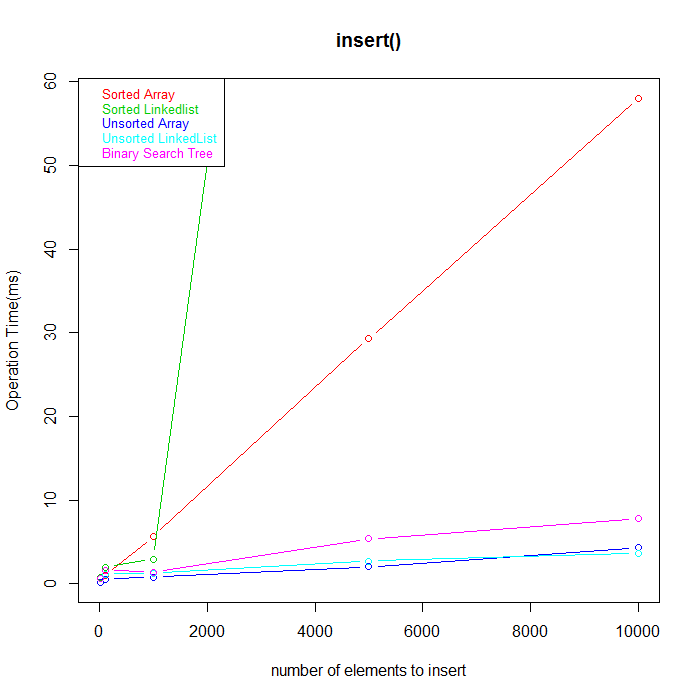
\includegraphics[scale = 0.5]{insert.png}
		\item \verb|find()|\\
			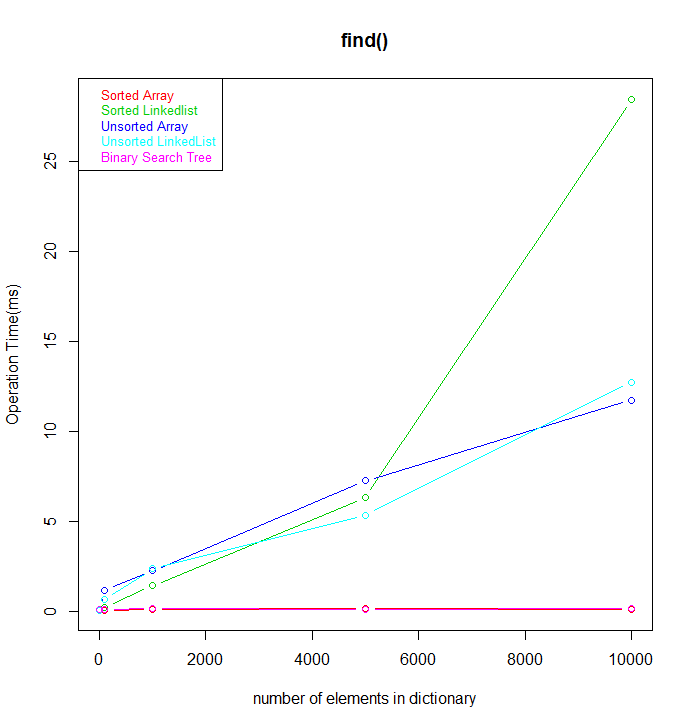
\includegraphics[scale = 0.5]{find.png}
		\item \verb|delete()|\\
			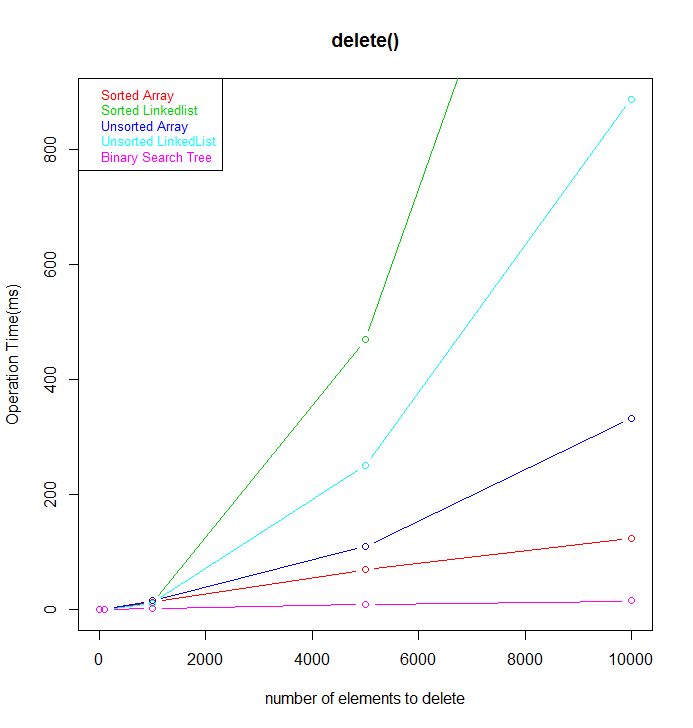
\includegraphics[scale = 0.5]{delete.png}
	\end{itemize}

	Use these graphs to answer the following questions.
	\question Which of the implementations seems to be the best overall? Explain why?
	\begin{itemize}
		\item BSTDict seems to be the best overall. Because for both \verb|find()| and \verb|delete()|, its runtime does not increase too much as size grows quickly. Although \verb|insert()| of BSTDict does not perform as well as UADict and ULLDict, it is still acceptable. 
		\item The reason why BSTDict has best performance is that, all of three functions have O(height) runtime on average.
	\end{itemize}
	\question Are there any surprising findings? Do all O(n) functions perform at the same speed? Why or why not?
	\begin{itemize}
		\item I am surprised that SLLDict performs so bad in \verb|find()| and \verb|delete()|.
		\item No, they do not. For example, for \verb|delete()|, SADict, SLLDict, UADict and ULLDict have O(n) runtime but the graph tells that as the size grows, operation time for each one grows at different speeds. 
	\end{itemize}


	\question Create inputs for the BSTDict to exhibit best case and worst case scenarios. Show the timing difference for the find function for large values of n.
	\\ The best case is when the tree is perfectly balanced. And the worst case is when the tree has all nodes in one single line.
	\begin{Verbatim}
	public class testBSTDict {
		private static final int N = 13;
		// size = 8191
		private static final int TEST_SIZE = (int)Math.pow(2, N) - 1;

		public static void main(String[] args) {
			BSTDict test1 = new BSTDict();
			BSTDict test2 = new BSTDict();
			bestCaseTest(test1);
			worstCaseTest(test2);
		}
		
		public static void bestCaseTest(BSTDict dict) {
			int n = (TEST_SIZE + 1) / 2;
			dict.insert(n, "dummy");
			add(dict, (int)Math.pow(2, N - 2), n);
			System.out.println("Best Case");
			System.out.println("Size" + "  " + "Time(ms)");
			findTester(dict);
		}
		
		private static void add(BSTDict dict, int diff, int n) {
			if (diff > 0) {
				dict.insert(n - diff, "dummy");
				dict.insert(n + diff, "dummy");
				add(dict, diff / 2, n - diff);
				add(dict, diff / 2, n + diff);
			}
		}
		
		public static void worstCaseTest(BSTDict dict1) {
			for (int i = 0; i < TEST_SIZE; i++) {
				dict1.insert(i, "");
			}
			System.out.println("Worst Case");
			System.out.println("Size" + "  " + "Time(ms)");
			findTester(dict1);
		}
		
		public static void findTester(BSTDict dict) {
			long startTime = System.nanoTime();
			int operations = 0;
			while(operations < 100) {
				dict.find(TEST_SIZE);
				operations++;
			}
			long endTime = System.nanoTime();
			System.out.print(TEST_SIZE + "  ");
			System.out.print((double)(endTime - startTime) / 1000000);
			System.out.println();
			System.out.println();
		}
	}
	\end{Verbatim}
	And this Code gives me the following result\\
	\begin{Verbatim}
		Best Case
		Size  Time(ms)
		8191  0.334617

		Worst Case
		Size  Time(ms)
		8191  4.824496

	\end{Verbatim}
	It can be seen that for large n, the time difference between best case and worst case is huge.


\end{questions}
\end{document}